\subsection{I metodi di Eulero in avanti e all'indietro}

Dato il problema di Cauchy, esso vale per ogni $t$ nell'intervallo $I$, quindi in particolare anche in $t_{n}$:
\begin{equation*}
	y'\left(t_{n}\right) = f\left(t_{n}, y\left(t_{n}\right)\right)
\end{equation*}
Approssimando la derivata sinistra con l'approssimazione in avanti introdotta a pagina \pageref{eq: approssimazione in avanti della derivata prima}, si ottiene:
\begin{equation*}
	D^{+} y\left(t_{n}\right) = \dfrac{y\left(t_{n+1}\right) - y\left(t_{n}\right)}{h} \approxeq f\left(t_{n}, y\left(t_{n}\right)\right)
\end{equation*}
Da notare che l'espressione assomiglia ad un'uguaglianza poiché l'espressione a sinistra è un'approssimazione della derivata e di conseguenza della funzione $f$.

\highspace
L'idea è quella di introdurre come soluzione numerica $u_{n}$ con $n = 1, \dots, N$ la quale è una successione di valori che risolve in maniera esatta la precedente relazione.
\begin{equation*}
	\begin{array}{rcl}
		\dfrac{y\left(t_{n+1}\right) - y\left(t_{n}\right)}{h} &\approxeq& f\left(t_{n}, y\left(t_{n}\right)\right) \\ [1em]
		%
		&\downarrow& \\ [.5em]
		%
		\dfrac{
			u_{n+1} - u_{n}
		}{h} &=& f\left(t_{n}, u_{n}\right)
	\end{array}
\end{equation*}
Da qui si ricava comodamente il \definition{metodo di Eulero in avanti}:
\begin{equation}\label{eq: metodo di Eulero in avanti}
	u_{n+1} = u_{n} + hf\left(t_{n}, u_{n}\right) \hspace{2em} n = 0, \dots, N - 1
\end{equation}

\highspace
In maniera analoga, partendo dal problema di Cauchy:
\begin{equation*}
	y'\left(t_{n+1}\right) = f\left(t_{n+1}, y\left(t_{n+1}\right)\right)
\end{equation*}
Approssimando la derivata a sinistra con l'approssimazione all'indietro introdotto a pagina \pageref{eq: approssimazione all'indietro della derivata prima}, si ottiene:
\begin{equation*}
	D^{-} y\left(t_{n+1}\right) = \dfrac{y\left(t_{n+1}\right) - y\left(t_{n}\right)}{h} \approxeq f\left(t_{n+1}, y\left(t_{n+1}\right)\right)
\end{equation*}
Introducendo una soluzione numerica $u_{n}$ con $n = 1, \dots, N$ la quale è una successione di valori che risolve in maniera esatta la precedente relazione.
\begin{equation*}
	\begin{array}{rcl}
		\dfrac{y\left(t_{n+1}\right) - y\left(t_{n}\right)}{h} &\approxeq& f\left(t_{n+1}, y\left(t_{n+1}\right)\right) \\ [1em]
		%
		&\downarrow& \\ [.5em]
		%
		\dfrac{
			u_{n+1} - u_{n}
		}{h} &=& f\left(t_{n+1}, u_{n+1}\right)
	\end{array}
\end{equation*}
Da qui si ricava comodamente il \definition{metodo di Eulero all'indietro}:
\begin{equation}\label{eq: metodo di Eulero all'indietro}
	u_{n+1} = u_{n} + hf\left(t_{n+1}, u_{n+1}\right) \hspace{2em} n = 0, \dots, N - 1
\end{equation}

\newpage
\begin{flushleft}
	\textcolor{Green3}{\faIcon{question-circle} \textbf{Perché il metodo di Eulero in avanti viene chiamato \underline{esplicito}?}}
\end{flushleft}
Per il metodo di Eulero in avanti, la condizione iniziale $u_{0} = y_{0}$ è ben nota. Dopodiché, viene effettuato un \textbf{calcolo in sequenza}, ovverosia $u_{1}$, $u_{2}$, e così via. Tuttavia, \underline{non} è un metodo iterativo poiché la soluzione è significativa per ogni $n$, essendo l'approssimazione della $y$ a diversi istanti temporali.

\highspace
Ovviamente i due metodi calcolano la nuova $u_{n+1}$ in modo differente. Infatti, il metodo di Eulero in avanti calcola:
\begin{equation*}
	u_{n+1} = u_{n} + hf\left(t_{n}, u_{n}\right)
\end{equation*}
Il \textbf{nuovo valore è calcolato in maniera esplicita}. Difatti è sufficiente valutare la funzione $f$, anche se non lineare, per $t_{n}$, $u_{n}$ ottenendo quindi un'espressione esplicita per il termine a destra. Questo è il motivo per cui il metodo di Eulero in avanti viene chiamato anche \definition{metodo di Eulero esplicito}.

\highspace
\begin{flushleft}
	\textcolor{Green3}{\faIcon{question-circle} \textbf{Perché il metodo di Eulero all'indietro viene chiamato \underline{implicito}?}}
\end{flushleft}
Per il metodo di Eulero all'indietro:
\begin{equation*}
	u_{n+1} = u_{n} + hf\left(t_{n+1}, u_{n+1}\right)
\end{equation*}
\textbf{Non si ha un'espressione esplicita} per il nuovo valore $u_{n+1}$ \textbf{perché quest'ultimo compare anche a destra dell'uguale}!

\highspace
Si pone come incognita $x = u_{n+1}$. Se la funzione $f$ non è lineare rispetto a $y$, allora ad ogni passo temporale è necessario risolvere il \definition{problema di ricerca degli zeri} della funzione:
\begin{equation}
	g\left(x\right) = x - u_{n} - hf\left(t_{n+1}, x\right)
\end{equation}
Se la funzione $g\left(x\right)$ è derivabile, allora è necessario introdurre ad ogni istante temporale un metodo iterativo, come quello di Newton per esempio. In ogni caso, a causa del fatto che $u_{n+1}$ non può in generale essere determinato per via esplicita, il metodo di Eulero all'indietro viene chiamato anche \definition{metodo di Eulero implicito}.


\highspace
In generale, si possono \textbf{dividere i metodi numerici} per le equazioni ordinarie in \textbf{metodi espliciti}, la cui \textbf{soluzione al nuovo passo temporale è calcolata mediante un'espressione esplicita}, e \textbf{metodi impliciti} che invece \textbf{richiedono la soluzione di un'equazione non lineare}.

\newpage

\subsubsection{Assoluta stabilità}

\begin{flushleft}
	\textcolor{Green3}{\faIcon{question-circle} \textbf{È stabile il metodo di Eulero?}}
\end{flushleft}
Per discutere della stabilità, è necessario introdurre il concetto di \definition{assoluta stabilità}. Un metodo numerico viene detto \textbf{assolutamente stabile} per un determinato valore di $h$ maggiore di zero, se:
\begin{equation}
	\left|u_{n+1}\right| \le C_{AS}\left|u_{n}\right| \hspace{2em} C_{AS} < 1
\end{equation}
O, equivalentemente, se si è su un intervallo illimitato:
\begin{equation*}
	\lim\limits_{n \rightarrow +\infty} \left|u_{n}\right| = 0
\end{equation*}
Adesso si analizzano i metodi singolarmente.

\highspace
\begin{flushleft}
	\textcolor{Red2}{\faIcon{bookmark} \textbf{Assoluta stabilità: metodo di Eulero in avanti}}
\end{flushleft}
Dato il \definition{problema modello lineare}:
\begin{equation*}
	\begin{cases}
		y'\left(t\right) = \lambda y\left(t\right) \hspace{2em} \lambda < 0 \\
		y\left(0\right) = 1
	\end{cases}
\end{equation*}
La cui soluzione esatta è: $y\left(t\right) = e^{\lambda t}$. Applicando il metodo di Eulero in avanti, si ottiene:
\begin{equation*}
	u_{n+1} = u_{n} + h\lambda u_{n} = \left(1+h\lambda\right)u_{n} \longrightarrow C_{AS} = \left|1 + h\lambda\right|
\end{equation*}
Da cui l'assoluta stabilità è \textbf{garantita se}:
\begin{equation*}
	C_{AS} < 1 \longrightarrow -1 < 1 + h\lambda < 1
\end{equation*}
Ovvero $h$ deve rispettare la seguente condizione:
\begin{equation}
	h\lambda > -2 \Rightarrow h < -\dfrac{2}{\lambda}
\end{equation}
Da notare che $h\lambda < 0$ è sempre vera.

\begin{examplebox}[: stabilità metodo di Eulero in avanti]
	Data la soluzione di un problema con $\lambda = -1$, ottenuto con il metodo di Eulero in avanti, nella seguente figura si può vedere come:
	\begin{itemize}
		\item Linea tratteggiata: rappresentata $h = \frac{30}{14}$. Quindi, essendo:
		\begin{equation*}
			h < -\dfrac{2}{\lambda} \Rightarrow \dfrac{30}{14} < -\dfrac{2}{-1} \Rightarrow \dfrac{30}{14} < 2 \:\: \text{\ding{55}}
		\end{equation*}
		La soluzione numerica oscilla e infine esplode.
		
		\item Linea continua: rappresentata $h = \frac{30}{16}$. Quindi, essendo:
		\begin{equation*}
			\dfrac{30}{16} < 2 \:\: \text{\ding{51}}
		\end{equation*}
		La soluzione numerica oscilla ma non esplode. La sua oscillazione è dovuta al fatto che è molto vicina al limite $2$.
		
		\item Linea tratto-punto: rappresentata $h = \frac{1}{2}$. Quindi, essendo:
		\begin{equation*}
			\dfrac{1}{2} < 2 \:\: \text{\ding{51}}
		\end{equation*}
		La soluzione numerica non oscilla.
	\end{itemize}
	\begin{center}
		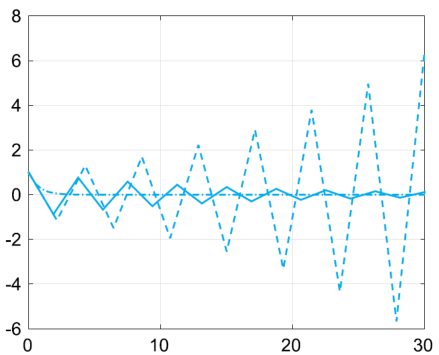
\includegraphics[width=.6\textwidth]{img/metodo-di-eulero-1.png}
	\end{center}
\end{examplebox}

\highspace
\begin{flushleft}
	\textcolor{Red2}{\faIcon{bookmark} \textbf{Assoluta stabilità: metodo di Eulero all'indietro}}
\end{flushleft}
Dato il solito problema modello lineare:
\begin{equation*}
	\begin{cases}
		y'\left(t\right) = \lambda y\left(t\right) \hspace{2em} \lambda < 0 \\
		y\left(0\right) = 1
	\end{cases}
\end{equation*}
La cui soluzione esatta è: $y\left(t\right) = e^{\lambda t}$. Applicando il metodo di Eulero all'indietro, si ottiene:
\begin{equation*}
	u_{n+1} = u_{n} + h\lambda u_{n+1} \rightarrow u_{n+1} = \dfrac{1}{1-h\lambda} u_{n} \rightarrow C_{AS} = \left|\dfrac{1}{1-h\lambda}\right|
\end{equation*}
In questo caso, l'\textbf{assoluta stabilità è \underline{sempre garantita}}, poiché:
\begin{equation*}
	C_{AS} < 1 \hspace{1em} \forall h
\end{equation*}
Quindi, per il metodo di Eulero all'indietro si può essere certi che è \textbf{incondizionatamente assolutamente stabile}.

\newpage

\subsubsection{Problemi di Cauchy generali}

Il concetto di stabilità introdotto nel paragrafo precedente riguarda il \emph{problema modello lineare}. Per cui, per i problemi di Cauchy, in generale, che stabilità si ha?

\highspace
\textbf{Un metodo numerico produce una soluzione stabile se a \emph{piccole} perturbazioni sul dato iniziale si producono perturbazioni \emph{piccole} e decrescenti per $n$ crescente.}

\highspace
Notando che per il \emph{problema modello lineare} si ha:
\begin{equation*}
	f\left(y\right) = \lambda y \: \rightarrow \: f'\left(y\right) = \lambda
\end{equation*}
Ha senso introdurre la \textbf{stima dell'intervallo dei valori} di $h$ che \underline{garantiscono} una \textbf{soluzione stabile} per il \textbf{\emph{metodo di Eulero in avanti}}:
\begin{equation}
	h < -\dfrac{2}{\overline{\lambda}} \hspace{3em} \overline{\lambda} = - \underset{t,y}{\max} \left|\dfrac{\partial f}{\partial y}\right| \hspace{3em} \dfrac{\partial f}{\partial y} < 0
\end{equation}
Essa rappresenta una situazione di cautela, la quale potrebbe essere molto restrittiva per il problema di Cauchy, ma sicuramente garantisce una soluzione numerica stabile.

\highspace
In generale, vale la proprietà che un \textbf{metodo numerico assolutamente stabile per il \emph{problema modello lineare}} sotto una condizione su $h$ (piccolo a sufficienza) \textbf{produce una soluzione numerica stabile anche per il problema di Cauchy generico sotto la stessa condizione opportunatamente adattata}.